
\chapter{Timeline of Time-Resolved Crystallography}
\label{ap: intro-timeline}

\newpage

\begin{figure}[hp!]
  \centering
  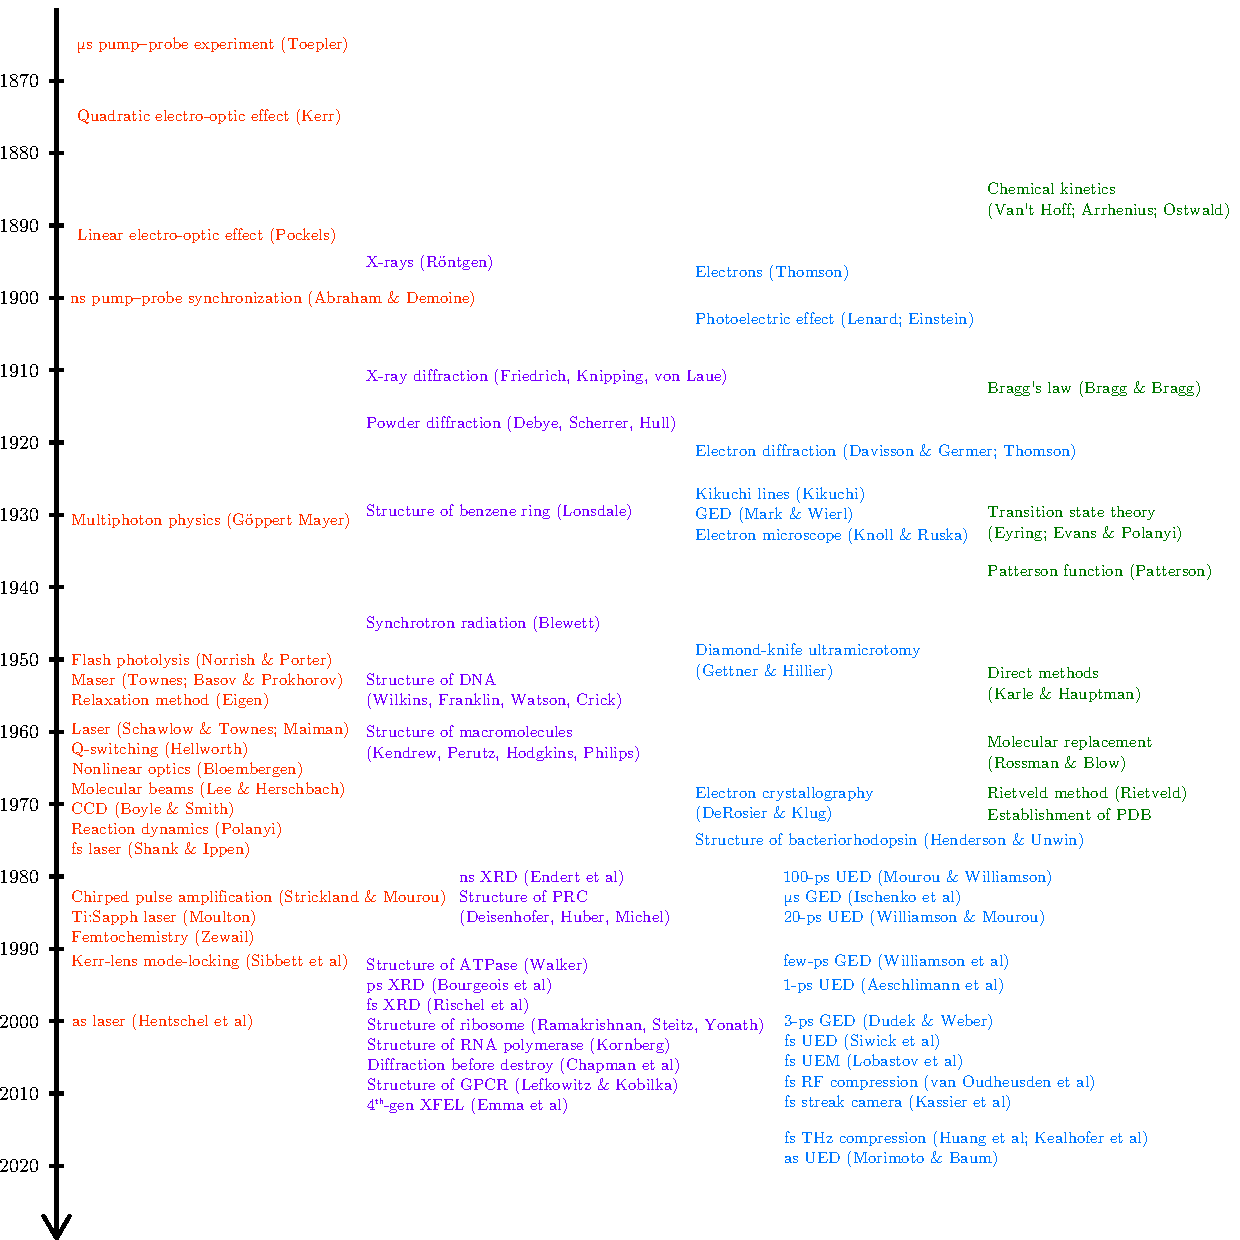
\includegraphics[width = \textwidth]{Figures/fig_intro_timeline.pdf}
  \caption[Timeline of time-resolved crystallography.]{
    Timeline of time-resolved crystallography:
    optics~(red), X-rays~(purple),
    electrons\protect\footnotemark\textsuperscript{,}\protect\footnotemark\textsuperscript{,}\protect\footnotemark~(blue),
    and theory~(green).
    Abbreviations:
    photosynthetic reaction centre~(PRC), G-protein-coupled receptors~(GPCR), Protein Data Bank~(PDB).
    gas-phase electron diffraction~(GED), ultrafast electron microscopy~(UEM).
    Dates and values are taken from Refs.~\cite{Pease1981, Villiger1990, Gehrenbeck1978,
    Glaeser1985, Glaeser1999, Bloembergen1999, Zewail2006, Califano2012, NatureMilestones,
    Hada2013, Ischenko2017} and the references therein.
  }
  \label{fig: intro-timeline}
\end{figure}

\addtocounter{footnote}{-3}

% Footnote 1
\stepcounter{footnote}
\footnotetext{
  As the first report of `ultrafast' electron diffraction,
  some authors~\cite{Hada2013, Ischenko2017}
  cite the 1983~work of Ischenko et~al~\cite{Ischenko1983}
  while others~\cite{Cao2003, Zewail2006} cite
  those of Mourou et~al~\cite{Mourou1982, Mourou1984}
  or Rood and Milledge~\cite{Rood1984} in 1982--1984.
}

% Footnote 2
\stepcounter{footnote}
\footnotetext{
  Note that the contemporary works of Siwick et~al~\cite{Siwick2003}
  and Cao et~al~\cite{Cao2003} can be distinguished as follows:
  the former reported on fs~structural dynamics associated with
  laser-induced melting of~{Al}
  and the latter observed ps~laser-driven lattice expansion of~{Ag}
  while both used fs~electron pulses.
}

% Footnote 3
% 120-fs laser pulse, 322-fs electron pulse, 6-14 mJ/cm2
\stepcounter{footnote}
\footnotetext{
  Unmarked here are the 2007 work of Baum et~al~\cite{Baum2007}
  on ps~UED in VO$_2$ under high laser excitation
  (ca. $6$--$14$~mJ/cm$^2$ or $50$--$117$~GW/cm$^2$)
  and some of Miller et~al that reported
  the first fs~RF-compressed UED experiments~\cite{Jean-Ruel2011, Jean-Ruel2013},
  including direct observations of atomic motions coupled to
  electron delocalization~\cite{Gao2013}
  and charge transfer~\cite{Ishikawa2015}.
}













%
